
\documentclass[10pt,landscape]{scrartcl}

\usepackage[english]{babel}
% \usepackage[ngerman]{babel}
\usepackage[utf8]{inputenc}

\usepackage{lmodern}

\usepackage{ifthen}

\usepackage{graphicx}
% \usepackage{pstricks}
% \usepackage{relsize}
% \usepackage[decimalsymbol=comma,exponent-product = \cdot, per=frac]{siunitx}
% \sisetup{range-phrase=\,bis\,}

\usepackage{xargs}
\usepackage{calc}
\usepackage{amsmath}
\usepackage{amsfonts}
\usepackage{mathtools}
\usepackage{amssymb}

\usepackage{cancel}
\usepackage{trfsigns}
\usepackage{array}
\usepackage{enumerate}
\usepackage{enumitem}

\usepackage{caption}
\usepackage{subcaption}

\usepackage{multicol}

\usepackage{pdflscape}
\usepackage[table]{xcolor}

\usepackage{float}

%%%%%%%%%%%%%%%%%%%%%%%%%%%%%%%%%%%%%%%%%%%%%%%%%%%%%%%%%%%%%%%%%%%%%%%%%%%%%%%%
\newboolean{WITHPSTRICKS}
\setboolean{WITHPSTRICKS}{false}


\newcommand{\PROFESSOR}{Prof.\ Dr.\ Thomas Carraro}
\newcommand{\ASSISTANT}{\setlength{\tabcolsep}{0pt}\begin{tabular}{l} M.Sc Janna Puderbach\end{tabular}}

\newcommand{\Jahr}{2024}
% \newcommand{\Trimester}{HT}
\newcommand{\Trimester}{WT}
\newcommand{\Kurs}{Mathematik II}
\newcommand{\TYPE}{Aufgabenblatt}
\newcommand{\BLATT}{1}
\newcommand{\TOPIC}{Definitheit, Ähnlichkeit}

%%%%%%%%%%%%%%%%%%%%%%%%%%%%%%%%%%%%%%%%%%%%%%%%%%%%%%%%%%%%%%%%%%%%%%%%%%%%%%%%
\newboolean{mitLoes}
\setboolean{mitLoes}{false}
% \setboolean{mitLoes}{true}

%%%%%%%%%%%%%%%%%%%%%%%%%%%%%%%%%%%%%%%%%%%%%%%%%%%%%%%%%%%%%%%%%%%%%%%%%%%%%%%%


%\setboolean{WITHPSTRICKS}{false}
%\setboolean{WITHPSTRICKS}{true}


\usepackage{tikz}
\usetikzlibrary{arrows,automata,backgrounds,calendar,decorations.pathmorphing,fadings,shadings,calc,intersections}
\usetikzlibrary{decorations.pathreplacing}
\usetikzlibrary{decorations.shapes}
\usetikzlibrary{decorations.footprints}
\usetikzlibrary{decorations.text}
\usetikzlibrary{positioning}
\usetikzlibrary{through}
\usepackage[utf8]{inputenc}


\ifthenelse{\boolean{WITHPSTRICKS}}{%
\usepackage{auto-pst-pdf}
\usepackage{pstricks,pst-plot,pst-text}
}{}

\usepackage{pgfplots}

%%%%%%%%%%%%%%%%%%%%%%%%%%%%%%%%%%%%%%%%%%%%%%%%%%%%%%%%%%%%%%%%%%%%%%%%%%%%%%%%
\usepackage{mbdefAufgaben}

%%%%%%%%%%%%%%%%%%%%%%%%%%%%%%%%%%%%%%%%%%%%%%%%%%%%%%%%%%%%%%%%%%%%%%%%%%%%%%%%
\newboolean{mitErg}
%\setboolean{mitErg}{false}

%%%%%%%%%%%%%%%%%%%%%%%%%%%%%%%%%%%%%%%%%%%%%%%%%%%%%%%%%%%%%%%%%%%%%%%%%%%%%%%%
\newcounter{Aufg}
\setcounter{Aufg}{0}
\newcounter{Blatt}
\setcounter{Blatt}{1}

%%%%%%%%%%%%%%%%%%%%%%%%%%%%%%%%%%%%%%%%%%%%%%%%%%%%%%%%%%%%%%%%%%%%%%%%%%%%%%%%
%\usepackage{KopfEnglish}

% Seitenraender
%\textwidth = 285mm
%\textheight = 180mm
%\leftmargin 5mm
%\oddsidemargin = -20mm
%\evensidemargin = -20mm
%\topmargin = -25mm
%\parindent 0cm
%\columnsep 2cm

% % % Aufgabenstellung
% % % Schwierungkeitsgrad mit "e" , "f" oder "v" angeben
% % % "e" Einführung   
% % % "f" Festigung
% % % "v" Vertiefung  

\newcommand{\Aufgabe}[3][]{
\stepcounter{Aufg}
\subsubsection*{Aufgabe 
\arabic{Aufg}\ifthenelse{\equal{#1}{e}}{}{\ifthenelse{\equal{#1}{f}}{
$\!\!{}^\star$}{\ifthenelse{\equal{#1}{v}}{$^{\star\star}$}{}}}{: #2}}
{#3}
}
% % % Ergebnisse jeweils am Ende des Aufgabenblattes Anzeigen
\newcommand{\Ergebnisse}{}
\makeatletter
\newcommand{\Ergebnis}[1]{
	\g@addto@macro{\Ergebnisse}{#1}
}
\makeatother
\makeatletter
\newcommand{\ErgebnisC}[2]{
\@ifundefined{c@#1}
{\newcounter{#1}}
{}
\setcounter{#1}{\theAufg}

\ifthenelse{\boolean{mitErg}}{	\g@addto@macro{\Ergebnisse}{\subsubsection*{Ergebnisse zu Aufgabe \arabic{#1}:}
}%
	\g@addto@macro{\Ergebnisse}{#2}}{}
}
\makeatother


% % % Lösungen
\newcommand{\Loesung}[1]{
	\ifthenelse{\boolean{mitLoes}}
	{\subsubsection*{Lösung \arabic{Aufg}:}
		#1}
	{}
}
% % % % % % % % % % % % % % % % % % % % % % % % % % % % % % % % % % % % % % % % % % % % % % % % % % % % % %
% % % % % % % % % % % % % % % % % % % % % % % % % % % % % % % % % % % % % % % % % % % % % % % % % % % % % %
% % % % % % % % % % % % % % % % % % % % % % % % % % % % % % % % % % % % % % % % % % % % % % % % % % % % % %
\begin{document}
%\begin{twocolumn}
% % % % % % % % % % % % % % % % % % % % % % % % % % %

%%%%%%%%%%%%%%%%%%%%%%%%%%%%%%%%%%%%%%%%%%%%%%%%%%%%%%%%%%%%%%%%%%%%%%%%%%%%%%%%
% Set the TITLE of the sheet here:
%\uebheader{\Kurs}{\arabic{Blatt}}{\Trimester\,\Jahr}{\TOPIC}
%\uebheader{\Kurs}{\arabic{Blatt}}{\Trimester\,\Jahr}{\TOPIC}
%\uebheader{\Kurs}{\arabic{Blatt}}{\Trimester\,\Jahr}{\TOPIC}
%\ruleBig

\setboolean{mitErg}{false}
 \setboolean{mitErg}{true}


%%%%%%%%%%%%%%%%%%%%%%%%%%%%%%%%%%%%%%%%%%%%%%%%%%%%%%%%%%%%%%%%%%%%%%%%%%%%%%%%
% Set the INTRODUCTION section of the sheet here:
% \input{introduction.tex}

\textbf{Einführende Bemerkungen}

\begin{itemize}
\item Vermeiden Sie die Verwendung von Taschenrechnern oder Online-Ressourcen.
\item Die mit einem Stern *) markierten (Teil-)Aufgaben entfallen in diesem Trimester. Stattdessen werden einzelne Online-Aufgaben im ILIAS-Kurs kenntlich gemacht, zu denen Sie dort Ihre L\"osungswege zur Korrektur hochladen k\"onnen. 
% \item Die mit zwei Sternen  **) markierten (Teil-)Aufgaben richten sich an Studierende, die die \"ubrigen Aufgaben bereits gel\"ost haben und die Inhalte weiter vertiefen m\"ochten. 
\end{itemize}

\ruleBig

%Mathe II Blatt 1

\Aufgabe[v]{Positive Definitheit}{
Welche der folgenden Matrizen ist positiv definit?
\begin{align*}
\text{ a)}&&\Vek A=&\begin{pmatrix}-1&2\\0&1\end{pmatrix},& \text{ b)}&&\Vek
B=&\begin{pmatrix}0&-1&0\\-1&0&0\\0&0&2\end{pmatrix}\\
\text{ c)}&&\Vek C =& \begin{pmatrix}1&1&1\\1&2&0\\1&0&3\end{pmatrix}&\text{ d)}&&\Vek
D=&\begin{pmatrix}\lambda&1&0\\1&1+\lambda&0\\0&0&1\end{pmatrix}\quad(\lambda\in\R)
\end{align*}

}

\Loesung{
\begin{abc}
\item $\Vek A$ ist nicht positiv definit, etwa mit $\Vek x=(1,-1)^\top$ ergibt sich: 
$$\Vek x^\top \Vek A \Vek x = (1,-1) \begin{pmatrix}-3\\-1\end{pmatrix}=-3+1=-2<0.$$
\item Mit $\Vek x=(1,0,0)^\top$ ergibt sich 
$$\Vek x^\top \Vek B \Vek x = (1,0,0)\begin{pmatrix}0\\-1\\0\end{pmatrix}=0.$$
Da aber f\"ur positive Definitheit mit allen $\Vek x\neq \Vek 0$ $\Vek x^\top\Vek B \Vek x >0$ gelten m\"usste, ist $\Vek B$
nicht positiv definit. 
\item Um positive Definitheit zu zeigen, muss f\"ur alle $\Vek x = (x_1,x_2,x_3)^\top\neq \Vek 0$
$\Vek x^\top C \Vek x>0$ \"uperpr\"uft werden: 
\begin{align*}
\Vek x^\top \Vek C \Vek x =& x_1^2 + 2 x_2^2 + 3x_3^2 + 2 x_1x_2 + 2 x_1x_3\\
=&\frac {x_1^2}2 + 2x_1x_2 + 2x_2^2 + \frac {x_1^2}2 + 2x_1x_3 + 2x_3^2+x_3^2\\
=&\left( \frac {x_1}{\sqrt 2} + \sqrt 2 x_2\right)^2 + \left( \frac{x_1}{\sqrt 2} + \sqrt 2
x_3\right)^2 + x_3^2
\end{align*}
Damit gilt auf jeden Fall $\Vek x^\top \Vek C \Vek x \geq 0$. Im Fall $\Vek x^\top \Vek C\Vek x=0$
m\"ussen beide Klammern des letzten Ausruckes und $x_3^2$ gleich Null sein. Daraus folgt dann
unmittelbar $x_3=0$ und (aus dem Verschwinden der zweiten Klammer) $x_1=0$ und damit (Verschwinden
der ersten Klammer) auch $x_2=0$. Insgesamt ist also nur f\"ur $\Vek x=0$ auch $\Vek x^\top \Vek C \Vek x
= 0$.\\
Damit ist $\Vek C$ positiv definit. 
\item Mit beliebigem $\Vek x\in\R^3$ gilt: 
\begin{align*}
\Vek x^\top \Vek D \Vek x =& \lambda x_1^2 + (1+\lambda)x_2^2 + x_3^2 + 2x_1x_2\\
=&(\sqrt \lambda x_1)^2 + 2\sqrt \lambda x_1 \cdot \frac{x_2}{\sqrt\lambda} + \frac{x_2^2}{\lambda}
+ \left( 1 + \lambda - \frac 1{\lambda}\right) x_2^2 + x_3^2\\
=&\left( \sqrt \lambda x_1 + \frac {x_2}{\sqrt \lambda}\right)^2 + x_3^2 + \frac {\lambda + \lambda^2
-1}\lambda x_2^2
\end{align*}
\begin{iii}
\item Falls $\frac{\lambda^2+\lambda-1}{\lambda}>0$, ist $\Vek x^\top \Vek D \Vek x\geq 0$ und nur f\"ur
$\Vek x=0$ ist $\Vek x^\top \Vek D\Vek x=0$, also ist $\Vek D$ positiv definit. 
\item Falls $\frac{\lambda^2+\lambda-1}{\lambda}<0$, ist f\"ur $\Vek x=(-1/\sqrt{\lambda},\sqrt\lambda,0)^\top$ $\Vek
x^\top\Vek D \Vek x<0$ und damit $\Vek D$ nicht positiv definit. 
\item Falls $\frac{\lambda^2+\lambda-1}{\lambda}=0$ ist, verschwindet $\Vek x^\top \Vek D \Vek x$
f\"ur $\Vek x=(-1/\sqrt\lambda,\sqrt\lambda,0)^\top\neq \Vek 0$, also ist $\Vek D$ nicht positiv definit. 
\item F\"ur $\lambda\leq 0$ ist obige Rechnung nicht m\"oglich, aber dann gilt\\
 $(1,0,0)\Vek D (1,0,0)^\top=\lambda\leq 0$ und $\Vek D$ ist nicht positiv definit. 
\end{iii}
Die Bedingungen f\"ur $\frac{\gamma_\lambda}{\lambda} := \frac{\lambda^2+\lambda-1}\lambda$ aus i)--iii) lassen sich weiter
umformen: \\
Zun\"achst ist der Z\"ahler 
$$\gamma_\lambda=\lambda^2+\lambda-1=(\lambda+\frac 12)^2-\frac 54$$
und hat seine Nullstellen bei $\frac {-1\pm \sqrt 5}2$. \\
Zwischen beiden Nullstellen ($\frac{-1-\sqrt 5}2 <\lambda<\frac{-1+\sqrt 5}2$) ist  $\gamma_\lambda<0$.\\
Au\ss erhalb des Intervals
($\lambda<\frac{-1-\sqrt 5}2$ oder $\lambda>\frac{-1+\sqrt 5}2$) ist $\gamma_\lambda>0$. 
Insgesamt ist also $\Vek D$ \\
positiv definit f\"ur  $\lambda>\frac{-1+\sqrt 5}2$ und  \\
nicht positiv definit f\"ur $\lambda\leq\frac{-1+\sqrt 5}2$.

\end{abc}
}

\ErgebnisC{AufglinalgPosiDefi001}
{
$\Vek A$ und $\Vek B$ sind nicht positiv definit, $\Vek C$ ist positiv definit. 

}

\ifthenelse{\boolean{mitLoes}}{\ruleBig \cleardoublepage}

% \Aufgabe[e]{Lineare Abbildungen}{
Gegeben seien die linearen Abbildungen $\vec f:\R^3\rightarrow \R^3$ und $\vec g: \R^3\rightarrow \R^2$ durch 
$$\vec f(x_1,x_2,x_3)=\begin{pmatrix} x_1-x_2\\
x_1+2x_3\\
x_1-x_2+x_3\end{pmatrix}\qquad\text{ und }\qquad\vec g(y_1,y_2,y_3)=\begin{pmatrix} y_2-y_3\\
y_1+y_2-y_3
\end{pmatrix}.$$
\begin{abc}
\item Geben Sie die Matrixdarstellungen der beiden linearen Abbildungen $\vec f$ und $\vec g$
sowie der Abbildung $\vec h=\vec g\circ \vec f$ an.
\item Bestimmen Sie mit Hilfe der Matrixdarstellungen aus Aufgabenteil \textbf{a)} $\vec f(1,1,-1)$, $\vec g(1,2,1)$ sowie $\vec h(1,1,-1)$. 
%\item Bestimmen Sie eine Basis des Kerns von $\vec g$. 
%\item Bestimmen Sie zudem $\vec f^{-1}(\Kern(\vec g))$. \\
%\textbf{Hinweis}: Beachten Sie die vorhergehende Teilaufgabe. 
%\item Geben Sie eine Basis von $\Kern(\vec g\circ \vec f)$ an. 
\end{abc}
}
\Loesung{
\begin{abc}
\item Die Abbildungsmatrix  der Abbildung $\vec f$ ist 
$$\vec A=\begin{pmatrix}
1  &  -1  &  0  \\
1  &   0  &  2  \\
1  &  -1  &  1  
\end{pmatrix},$$ 
die der Abbildung $\vec g$: 
$$\vec B=\begin{pmatrix}
0 & 1 & -1 \\
1 & 1 & -1\end{pmatrix}.$$
Die Abbildung $\vec h$ hat die Darstellung: 
\begin{align*}
\vec h(x_1,x_2,x_3)=&\vec g(\vec f(x_1,x_2,x_3))\\
=& \begin{pmatrix}f_2(x_1,x_2,x_3)-f_3(x_1,x_2,x_3)\\
f_1(x_1,x_2,x_3)+f_2(x_1,x_2,x_3)-f_3(x_1,x_2,x_3)\end{pmatrix}\\
=& \begin{pmatrix}
x_1+2x_3-(x_1-x_2+x_3)\\
x_1-x_2 + (x_1+2x_3) - (x_1-x_2+x_3)
\end{pmatrix}
= \begin{pmatrix}
x_2+x_3\\
x_1+x_3
\end{pmatrix}
\end{align*}
Damit hat $\vec h(\vec x)$ die Matrixdarstellung 
$$\vec C=\begin{pmatrix} 0 &1 & 1\\ 1 & 0 & 1\end{pmatrix}.$$

Alternativ kann man die  Matrix der verketteten Abbildung auch als Produkt der Abbildungsmatrizen berechnen: 
$$\vec B\vec A = \begin{pmatrix}
0  &  1  &  1 \\
1  &  0  &  1\end{pmatrix}.$$
\item Es sind
\begin{align*}
&&\vec f(1,1,-1)=& \vec A\begin{pmatrix} 1\\1\\-1\end{pmatrix}= \begin{pmatrix}0\\-1\\-1\end{pmatrix}\\
&&\vec g(1,2,1)=& \vec B \begin{pmatrix} 1\\2\\1\end{pmatrix} = \begin{pmatrix}1\\2\end{pmatrix}\\
&&\vec h(1,1,-1)=& \vec C \begin{pmatrix} 1\\1\\-1\end{pmatrix} = \begin{pmatrix}0\\0\end{pmatrix}.
\end{align*}
%\item Gem\"aß Dimensionssatz f\"ur lineare Abbildungen hat der Kern der Abbildung $\vec g$ die Dimension: 
%$$\dim(\Kern(\vec B))=3-\text{Rang }\vec B = 3-2=1$$
%Nach der vorhergehenden Aufgabe wird $\Kern (\vec g)$ also aufgespannt durch den Vektor $(0,-1,-1)^\top$. 
%\item $\vec f^{-1}(\Kern(\vec g))$ ist die Vereinigung der L\"osungsmengen der Gleichungen 
%$$\vec A \vec x = t\begin{pmatrix}0\\-1\\-1\end{pmatrix},\qquad t\in\R.$$ 
%Da $\vec A$ den Rang 3 hat, ist dieses Gleichungssystem f\"ur festes $t$ eindeutig l\"osbar. Die L\"osung ist dann (mit Hilfe von Aufgabe \textbf{b)}: 
%$$\vec x=t\begin{pmatrix}1\\1\\-1\end{pmatrix}$$
%Folglich ist 
%$$\vec f^{-1}(\Kern(\vec g))=\Span\{(1,1,-1)^\top\}.$$
%\item Es ist gerade $\Kern(\vec g\circ \vec f)=\vec f^{-1}(\Kern(\vec g))$. Somit ist $(1,1,-1)^\top$ eine Basis des Kerns von $\vec g\circ \vec f$. 
\end{abc}
}


\ErgebnisC{linalg_Abbi_Klau_01b}
{
\textbf{b)} \begin{align*}
\vec f(1,1,-1)=& \begin{pmatrix}0\\-1\\-1\end{pmatrix},\, 
&\vec g(1,2,1)=&  \begin{pmatrix}1\\2\end{pmatrix},\, 
&\vec h(1,1,-1)=& \begin{pmatrix}0\\0\end{pmatrix}
\end{align*}
}

% \ifthenelse{\boolean{mitLoes}}{\ruleBig \cleardoublepage}

\Aufgabe[f]{Lineare Abbildung im Komplexen}{
Gegeben ist die lineare Abbildung $\Vek L: \, \C^4 \, \rightarrow \, \C^3$ mit der Matrix 
$$\Vek A = \begin{pmatrix} 
    1 &  1+\imag &        1 &    \imag \\ 
    0 &        1 &        1 &        1 \\ 
    1 &   2\imag &    \imag &  2\imag-1
\end{pmatrix}$$
sowie der Vektor $\Vek b_\lambda = (\lambda-\imag, \, 0,\, -2\imag)^\top.$
\begin{abc}
\item Geben Sie $\Rang (\Vek A)$ und Orthonormalbasen von $\Bild \Vek A$ sowie $\Kern\Vek A$ und
  $(\Bild \Vek A)^\perp$ an. 
\end{abc}
\textbf{Hinweise}: 
\begin{itemize}
\item Der Orthogonalraum $\vec U^\perp$ eines Unterraumes $\vec U\subset\C^n$ enth\"alt alle Vektoren, die senkrecht zu allen
Vektoren aus $\vec U$ sind: 
$$\vec U^\perp=\{\vec v\in\C^n|\, \skalar{\vec v,\vec u}=0\text{ f\"ur alle }\vec u\in\vec U\}$$
\item Im Komplexen gilt $(\Bild\vec A)^\perp = \Kern(\vec A^*)$. 
\end{itemize}
\begin{abc}\setcounter{enumi}{1}
\item F\"ur welche $\lambda\in \C$ ist $\Vek b_\lambda\in \Bild\Vek A$ enthalten?
\item Geben Sie f\"ur beliebige $\lambda\in\C$ eine Zerlegung von $\Vek b_\lambda$ in Komponenten
  aus $\Bild \Vek A$ und $(\Bild \Vek A)^\perp$ an. 
\item Bestimmen Sie alle $\Vek x_\lambda\in \C^4$, so dass $\Vek A \Vek x_\lambda$ die orthogonale
  Projektion von $\Vek b_\lambda$ auf $\Bild \Vek A$ ist. 
\end{abc}


}

\Loesung{
\begin{abc}
\item Um eine Basis von $\Bild \Vek A$ zu bestimmen, wenden wir den Gauß-Algorithmus auf die
Spaltenvektoren von $\Vek A$ an: 
$$\begin{array}{rrr|l}
       1  &       0 &       1  & \text{                                    }\\
  1+\imag &       1 &   2\imag & \text{ -$(1+\imag)\cdot$ 1. Zeile         }\\
       1  &       1 &    \imag & \text{ -1. Zeile                          }\\
    \imag &       1 & 2\imag-1 & \text{ -$\imag\cdot$ 1. Zeile             }\\\hline

       1  &       0 &       1  & \text{                                    }\\
       0  &       1 & -1+\imag & \text{                                    }\\
       0  &       1 & \imag-1  & \text{ -2. Zeile                          }\\
       0  &       1 & \imag-1  & \text{ -2. Zeile                          }\\\hline

       1  &       0 &       1  & \text{                                    }\\
       0  &       1 & -1+\imag & \text{                                    }\\
       0  &       0 &       0  & \text{                                    }\\
       0  &       0 &       0  & \text{                                    }
\end{array}$$
Eine Basis des Bildraumes ist damit 
$$\{(1,\, 0,\, 1)^\top, \, (0,\, 1,\, \imag-1)^\top\}.$$
Diese wird noch orthonormiert: 
\begin{align*}
&&\Vek v_1 = & \frac 1{\sqrt 2} (1,\, 0,\, 1)^\top\\
&&\Vek w_2 = & (0,\, 1,\, \imag-1)^\top - \frac 12 \skalar{(0,\, 1,\, \imag-1)^\top,\, (1,\, 0,\, 1)^\top} (1,\, 0,\, 1)^\top\\
&&=& \frac 12 (1-\imag ,\, 2,\, \imag-1)^\top\\
\Rightarrow &&\Vek v_2 = & \frac 1 {\sqrt{8}} (1-\imag,\, 2,\, \imag-1)^\top
\end{align*}
Die Vektoren $\vec v_1$ und $\vec v_2$ bilden eine Basis von $\Bild \vec A$. Um eine Basis des
Orthogonalraumes $(\Bild \vec A)^\perp$ zu erhalten, setzen wir den Gram-Schmidt-Algorithmus mit einem
willk\"urlichen Vektor -- hier $\vec e_3$ -- fort: 
\begin{align*}
&&\vec w_3=&\vec e_3 -  \skalar{\vec e_3,\, \vec v_1} \vec v_1 - \skalar{\vec e_3,\, \vec v_2}\vec
v_2\\
&&=& \begin{pmatrix}0\\0\\1\end{pmatrix} - \frac 12 \begin{pmatrix}1\\0\\1\end{pmatrix} - \frac
{-1-\imag}8 \begin{pmatrix}1-\imag \\ 2 \\\imag -1\end{pmatrix}
= \frac 14 \begin{pmatrix} -1\\1+\imag\\1\end{pmatrix}\\
\Rightarrow&&\vec v_3 = & \frac 12 \begin{pmatrix}-1\\1+\imag\\1\end{pmatrix}
\end{align*}
Dieser Vektor $\vec v_3$ bildet eine Orthonormalbasis von $(\Bild\vec A)^\perp$. 

Der Rang der Abbildung ist 2. Gem\"aß Dimensionsformel hat der Kern somit die Dimension $4-2=2$. 
Wir ermitteln ihn im Gauß-Verfahren: 
$$\begin{array}{rrrr|r|l}
       1 &  1+\imag &        1 &  \imag   &        0 & \text{                            }\\
       0 &       1  &        1 &       1  &        0 & \text{                            }\\
       1 &   2\imag &  \imag   & 2\imag-1 &        0 & \text{ -1. Zeile                  }\\\hline

       1 &  1+\imag &        1 &  \imag   &        0 & \text{                            }\\
       0 &       1  &        1 &       1  &        0 & \text{                            }\\
       0 &  \imag-1 &  \imag-1 &  \imag-1 &        0 & \text{ -$(\imag-1)\cdot$ 2. Zeile }\\\hline

       1 &  1+\imag &        1 &  \imag   &        0 & \text{                            }\\
       0 &       1  &        1 &       1  &        0 & \text{                            }\\
       0 &       0  &        0 &       0  &        0 & \text{ -$(\imag-1)\cdot$ 2. Zeile }
\end{array}$$
Wir w\"ahlen zun\"achst $(x_3,x_4)=(1,0)$, um den ersten Basisvektor $(\imag,\, -1,\, 1,\, 0)^\top$
und dann $(x_3,x_4)=(0,1)$, um den zweiten Basisvektor $(1,\, -1,\, 0,\, 1)^\top$ zu erhalten. F\"ur diese
beiden Vektoren liefert das Schmidtsche Verfahren: 
\begin{align*}
&&\Vek z_1 = & \frac 1{\sqrt 3} (\imag,\, -1,\, 1,\, 0)^\top\\
&&\Vek z'_2 = & (1,\, -1,\, 0,\, 1)^\top - \frac 13 (-\imag+1) (\imag,\, -1,\, 1,\, 0)^\top=\frac 13
( 2-\imag,\, -2-\imag,\, \imag-1,\, 3)^\top\\
\Rightarrow &&\Vek z_2 = & \frac 1{\sqrt{21}} (2-\imag,\, -2-\imag,\, \imag -1,\, 3)^\top
\end{align*}

\item Es ist $\Vek b_\lambda\in \Bild \Vek A$, wenn $\{\Vek b_\lambda,\, \Vek v_1,\, \Vek v_2\}$
linear abh\"angig ist. Dies pr\"ufen wir mittels Gauß-Verfahren nach: 
$$\begin{array}{rrr|l}
       1       &       0  &       1 & \text{(Vielfaches von $\Vek v_1$)           }\\
 1-\imag       &       2  & \imag-1 & \text{(Vielfaches von $\Vek v_2$)           }\\
 \lambda-\imag &       0  & -2\imag & \text{($\Vek b_\lambda$)                     }\\\hline

       1       &       0  &       1         & \text{}\\
       0       &       2  & 2 \imag-2       & \text{2. Zeile - $(1-\imag)\cdot$ 1. Zeile    }\\
       0       &       0  & -\lambda-\imag  & \text{3. Zeile - $(\lambda-\imag)\cdot$ 1. Zeile}
\end{array}$$
Die letzte Zeile verschwindet genau dann, wenn $\lambda=-\imag$ ist, dann sind die drei Vektoren
linear abh\"angig, es ist also 
$$\Vek b_{-\imag}\in \Bild \Vek A.$$
\item Die Projektion auf $\Bild \Vek A$ wird geliefert durch 
\begin{align*}
\Vek P ( \Vek b_\lambda) = &\skalar{\Vek b_\lambda,\Vek v_1}\Vek v_1 + \skalar{\Vek b_\lambda,\Vek
v_2}\Vek v_2\\
=& \frac{\lambda-3\imag}{2}\begin{pmatrix}1\\0\\1\end{pmatrix}
+ \frac{\lambda(1+\imag)-1+\imag}8\begin{pmatrix}1-\imag\\2\\\imag-1\end{pmatrix}\\
=& \frac \lambda{8} \begin{pmatrix} 6\\2+2\imag\\2\end{pmatrix}+\frac
18\begin{pmatrix} -10\imag\\-2+2\imag\\-14\imag\end{pmatrix}
=\frac \lambda 4 \begin{pmatrix} 3\\1+\imag\\1\end{pmatrix}
 - \frac 14\begin{pmatrix}5\imag\\1-\imag\\7\imag\end{pmatrix}.
\end{align*}
Der Anteil von $\Vek b_\lambda$  orthogonal zu $\Bild \Vek A$ ergibt sich als Differenz aus beiden: 
\begin{align*}
\Vek b_\lambda - \Vek P(\Vek b_\lambda) =
& \frac{\lambda}{4}\begin{pmatrix}1\\-1-\imag\\-1\end{pmatrix} 
+ \frac 14\begin{pmatrix}\imag\\1-\imag\\-\imag\end{pmatrix}.
\end{align*}
\item Es soll also gelten $\Vek A \Vek x_\lambda = \Vek P (\Vek b_\lambda)$: 
$$\begin{array}{rrrr|r}
1       &1+\imag   &1       & \imag  & 3/4\lambda - 5/4\imag\\
0       &1         &1       &    1   & (1+\imag)/4\lambda - (1-\imag)/4\\
1       &2\imag    &\imag   &2\imag-1& 1/4\lambda - 7/4\imag\\\hline

1       &1+\imag   &1       & \imag  & 3/4\lambda - 5/4\imag\\
0       &1         &1       &    1   & (1+\imag)/4\lambda - (1-\imag)/4\\
0       &1-\imag   &1-\imag &1-\imag & \lambda/2  + 1/2\imag\\\hline

1       &1+\imag   &1       & \imag  & 3/4\lambda - 5/4\imag\\
0       &1         &1       &    1   & (1+\imag)/4\lambda - (1-\imag)/4\\
0       &0         &0       & 0      &      0                       
\end{array}$$
Dies liefert die Partikul\"arloesung 
$$\Vek x_\lambda^0=((2-i)/4\lambda + (1-6\imag)/4,\, 0,\,
(1+i)/4\lambda - (1-i)/4,\, 0)^\top$$
 und damit die allgemeine L\"osung: 
$$\Vek x_\lambda\in \Vek x_\lambda^0+\Kern(\Vek A).$$
\end{abc}
}

\ErgebnisC{AufglinalgAbbiKmpl001}
{
\textbf{ a)} $\Rang(\Vek A)=2$, $\Bild(\Vek A) = \Spn\{(1/\sqrt{2},0,1/\sqrt{2})^\top, \, 1/\sqrt{8}(1-\imag,\,
2,\, \imag-1)^\top\}$,\\
$\Kern(\Vek A) = \Spn \{1/\sqrt{3}(\imag,-1,1,0)^\top,\, 1/\sqrt{21}(2-\imag, -2-\imag, \imag
-1, 3)^\top\}$\\
\textbf{ b)} $\Vek b_{-i}\in\Bild(\Vek A)$
}

\ifthenelse{\boolean{mitLoes}}{\ruleBig \cleardoublepage}

\Aufgabe[e]{Determinanten}{
Bestimmen Sie die Determinante der folgenden Matrix mit Hilfe des Gau\ss{}'schen
Algorithmus:
$$\boldsymbol B = 
	\begin{pmatrix}
	 1 &  2 &  1 & -3 &  0 \\
	-3 & -6 & -4 &  7 &  1 \\
	 2 &  5 &  3 & -5 &  2 \\
	-3 & -8 & -2 &  7 &  3 \\
	 0 &  2 &  1 &  6 &  3
	\end{pmatrix}
$$
}
\Loesung{
\begin{align*}
\operatorname{det} \boldsymbol B & = \operatorname{det}
	\begin{pmatrix}
	 1 &  2 &  1 & -3 &  0 \\
	 0 &  0 & -1 & -2 &  1 \\
	 0 &  1 &  1 &  1 &  2 \\
	 0 & -2 &  1 & -2 &  3 \\
	 0 &  2 &  1 &  6 &  3
	\end{pmatrix} \quad &(\text{tausche } Z_2 \text{ und } Z_3)\\
	& = -1\cdot\operatorname{det}
	\begin{pmatrix}
	 1 &  2 &  1 & -3 &  0 \\
	 0 &  1 &  1 &  1 &  2 \\
	 0 &  0 & -1 & -2 &  1 \\
	 0 & -2 &  1 & -2 &  3 \\
	 0 &  2 &  1 &  6 &  3
	\end{pmatrix}&(Z_4 + 2 \cdot Z_2;\; Z_5 - 2 \cdot Z_2)\\
	& = -1\cdot\operatorname{det}
	\begin{pmatrix}
	 1 &  2 &  1 & -3 &  0 \\
	 0 &  1 &  1 &  1 &  2 \\
	 0 &  0 & -1 & -2 &  1 \\
	 0 &  0 &  3 &  0 &  7 \\
	 0 &  0 & -1 &  4 & -1
	\end{pmatrix} &(Z_4 + 3 \cdot Z_3;\; Z_5 - Z_3)\\
	& = -1\cdot\operatorname{det}
	\begin{pmatrix}
	 1 &  2 &  1 & -3 &  0 \\
	 0 &  1 &  1 &  1 &  2 \\
	 0 &  0 & -1 & -2 &  1 \\
	 0 &  0 &  0 & -6 & 10 \\
	 0 &  0 &  0 &  6 & -2
	\end{pmatrix}&(Z_5 + Z_4)\\
	& = -1\cdot\operatorname{det}
	\begin{pmatrix}
	 1 &  2 &  1 & -3 &  0 \\
	 0 &  1 &  1 &  1 &  2 \\
	 0 &  0 & -1 & -2 &  1 \\
	 0 &  0 &  0 & -6 & 10 \\
	 0 &  0 &  0 &  0 &  8
	\end{pmatrix}\\ 
	& = (-1)\cdot 1\cdot 1\cdot(-1)\cdot(-6)\cdot 8 = -48\ .	
\end{align*}

}

\ErgebnisC{dummy001}
{
{a)} $\operatorname{det}\boldsymbol B = -48 $
}

\ifthenelse{\boolean{mitLoes}}{\ruleBig \cleardoublepage}

\input{../A/Lineare_Algebra/licdnalg_Detn_Lapl_001.tex}
\ifthenelse{\boolean{mitLoes}}{\ruleBig \cleardoublepage}
% 
\Aufgabe[e]{\"Ahnlichkeitstransformation}{

Gegeben sind 
$$\Vek A =  \begin{pmatrix} 2& 0& 4\\0&6&0\\4&0&2\end{pmatrix}, \, \Vek a = \begin{pmatrix}
1\\\alpha\\-1\end{pmatrix}\text{ und } \Vek b = \begin{pmatrix}\beta\\ -\beta\\1\end{pmatrix}.$$
\begin{abc}
\item Bestimmen Sie -- wenn m\"oglich -- $\alpha$ und $\beta$ so, dass $\Vek a$ und $\Vek b$
Eigenvektoren der Matrix $\Vek A$ sind. 
\item Berechnen Sie einen weiteren (linear unabh\"angigen) Eigenvektor nebst zugeh\"origem
Eigenwert. 
\item Bestimmen Sie  orthogonale Matrizen $\Vek Q_i$, sowie Diagonalmatrizen $\Vek D_i$ ($i=1,2,3$),
so dass gilt
$$\Vek D_i = \Vek Q_i^\top \Vek B_i \Vek Q_i, \qquad i=1,2,3.$$
Dabei sind $\Vek B_1=\Vek A$, $\Vek B_2=\Vek A^{-1}$ und $\Vek B_3=\Vek A^3$. 
\end{abc}

}

\Loesung{
\begin{abc}
\item Es gilt
$$\Vek A \Vek a = \Vek A \begin{pmatrix}1\\\alpha\\-1\end{pmatrix}=\begin{pmatrix}
-2\\6\alpha\\2\end{pmatrix}. $$
Wenn $\Vek a$ Eigenvektor ist, folgt aus der ersten und dritten Komponente der Gleichung der
Eigenwert $-2$. F\"ur die zweite Komponente gilt dann $6\alpha \overset != -2\alpha$, also
$\alpha=0$. \\
F\"ur den zweiten Vektor $\Vek b$ hat man
$$\Vek A \Vek b = \Vek A \begin{pmatrix} \beta\\-\beta \\1 \end{pmatrix} 
= \begin{pmatrix} 2\beta+4\\ -6\beta \\ 4\beta + 2\end{pmatrix}$$
Wir nehmen erneut an, dass $\Vek b$ ein Eigenvektor ist. \\
F\"ur $\beta\neq 0$ w\"are der zugeh\"orige Eigenwert $\lambda=6$. (2. Komponente der Gleichung)\\
Aus der ersten Komponente der Gleichung folgt damit $6\beta=2\beta + 4$, also $\beta = 1$\\
Aus der dritten Komponente folgt $6=4\beta + 2$, also $\beta=1$.\\
Damit ist f\"ur $\beta=1$ $\Vek b= (1,-1,1)^\top$ ein Eigenvektor von $\Vek A$ mit dem Eigenwert $6$. 
\item Allgemein ergeben sich die Eigenwerte von $\Vek A$ als Nullstellen des charakteristischen
Polynoms: 
\begin{align*}
&&0\overset !=& \det\begin{pmatrix}
2-\lambda &           0 &            4 \\
        0 & 6-\lambda   &            0 \\
        4 &           0 & 2-\lambda    \end{pmatrix}
= (6-\lambda)\det\begin{pmatrix}
2-\lambda &           4 \\
        4 & 2-\lambda   \end{pmatrix}\\
&&=& (6-\lambda)((2-\lambda)^2-16)\\
\Rightarrow &&\lambda\in& \{-2,\, 6,\, 6\}
\end{align*}
Ein Eigenvektor zum Eigenwert $6$ ist L\"osung von 
$$0\overset != (\Vek A-6\Vek E ) \Vek c = \begin{pmatrix}-4&0&4\\0&0&0\\4&0&-4\end{pmatrix} \Vek
c.$$
Das Gleichungssystem hat den Rang 1, die geometrische Vielfachheit des Eigenwertes $6$ ist also
gleich der algebraischen Vielfachheit $2$. \\
Es ergeben sich die beiden linear unabh\"angigen L\"osungen $\Vek c = (1,\, 0,\, 1)^\top$
und $\Vek d = (0,\, 1,\, 0)^\top$. (Der Vektor $\Vek b$ ist im Eigenraum zu $\lambda=6$ enthalten:
$\Vek b = \Vek c - \Vek d$.)
\item Zur Diagonalisierung von $\Vek B_1=\Vek A$ stellt man die Matrix der normierten Eigenvektoren
auf: 
$$\Vek Q = \left( \frac{\Vek a}{\norm{\Vek a}}, \, \frac{\Vek c}{\norm{\Vek c}},\, \frac{\Vek
                           d}{\norm{\Vek d}}\right)=\begin{pmatrix} 1/\sqrt{2} & 1/\sqrt{2} & 0\\
                           0          & 0          & 1\\
                           -1/\sqrt 2 & 1/\sqrt{2} & 0\end{pmatrix}.$$
Die Diagonale von $\Vek D_1$ enth\"alt dann die Eigenwerte von $\Vek A$:
$$\Vek D_1 = \begin{pmatrix} -2 & 0 & 0\\0 & 6 & 0\\0& 0 & 6\end{pmatrix}.$$
$\Vek B_2=\Vek A^{-1}$ hat dieselben Eigenvektoren wie $A$, somit erh\"alt man mit derselben
Transformationsmatrix $\Vek Q_2=\Vek Q_1$ die Diagonalmatrix der Eigenwerte von $\Vek A^{-1}$: 
$$\Vek D_2 = \begin{pmatrix} -1/2&0&0\\ 0&1/6&0\\ 0&0&1/6 \end{pmatrix}.$$
Auch $\Vek B_3 = \Vek A^3$ hat dieselben Eigenvektoren $\Vek v\in\{\Vek a,\Vek c,\Vek d\}$:
$$\Vek A^3 \Vek v = \Vek A^2 \lambda \Vek v = \lambda \Vek A \lambda \Vek v = \lambda^2 \lambda \Vek
v = \lambda^2\Vek v.$$
Es ist also $\Vek Q_3 = \Vek Q_1$ und die zugeh\"orige Diagonalmatrix enth\"alt die dritte Potenz
der Eigenwerte von $\Vek A$: 
$$\Vek D_3 = \begin{pmatrix} -8 & 0 & 0\\ 0 & 36 & 0\\ 0 & 0 & 216\end{pmatrix}. $$
\end{abc}

}


\ErgebnisC{AufglinalgMatrSymm003}
{
\textbf{b)} $\lambda\in\{-2,\, 6\}$, $\Vek v_1 = (1,0,-1)^\top$, $\Vek v_2 = (1,0, 1)^\top$, $\Vek v_3
= (0,1, 0)^\top$

}

\ifthenelse{\boolean{mitLoes}}{\ruleBig \cleardoublepage}


\Aufgabe[e]{Symmetrische Matrizen}{
\begin{abc}
\item Bestimmen Sie mit Hilfe des Gaußschen Algorithmus die inverse Matrix von
$$ \Vek  A = \begin{pmatrix}
	 2 & -1 &  0 \\
	-1 &  2 & -1 \\
	 0 & -1 &  2 
\end{pmatrix}.$$


\item  Ist $\Vek A^{-1}$ wieder symmetrisch? Gilt diese Aussage f\"ur beliebige invertierbare symmetrische Matrizen?
\end{abc}

}

\Loesung{
\begin{abc}
\item Das Eliminationsverfahren ergibt
$$\begin{array}{rrr|rrr|l}
	 2 & -1 &  0 & 1 & 0 & 0 \\      
	-1 &  2 & -1 & 0 & 1 & 0       & \text{ + 1/2 $\cdot$ 1. Zeile   }\\     
	 0 & -1 &  2 & 0 & 0 & 1 \\\hline

	 2 & -1 &  0      &  1 & 0 & 0 \\    
	 0 & \frac 32 & -1&  \frac 12 & 1 & 0\\
	 0 & -1 &  2      &  0 & 0 & 1       & \text{ + 2/3 $\cdot$ 2. Zeile   }\\\hline

         2 & -1 &  0      &  1 & 0 & 0               & \text{                          }\\    
	 0 & \frac 32 & -1&  \frac 12 & 1 & 0        & \text{ + 3/4 $\cdot$ 3. Zeile   }\\          
	 0 & 0 & \frac 43 &  \frac 13 & \frac 23 & 1 & \text{       $\cdot$ 3/4        }\\\hline

	 2 & -1 &  0      &  1 & 0 & 0                      & \text{ + 2/3 $\cdot$ 2. Zeile   }\\
	 0 & \frac 32 & 0 &  \frac 34 & \frac 64 & \frac 34 & \text{ $\cdot$ 2/3              }\\
	 0 & 0 & 1 \      &  \frac 14 & \frac 24 & \frac 34 & \text{                          }\\\hline

	 2 & 0 &  0       &  \frac 64 & 1 & \frac 24  & \text{ $\cdot$ 1/2  }\\      
	 0 & 1 & 0        &  \frac 12 & 1 & \frac 12 \\      
	 0 & 0 & 1        &  \frac 14 & \frac 12 & \frac 34 \\\hline

	 1 & 0 &  0       &  \frac 34 & \frac 12 & \frac 14 \\ 
	 0 & 1 & 0        &  \frac 12 & 1 & \frac 12 \\        
	 0 & 0 & 1        &  \frac 14 & \frac 12 & \frac 34 
\end{array}$$

Die Inverse Matrix lautet also
$$ \Vek A^{-1} = \frac 14 \begin{pmatrix}
	 3 & 2 & 1 \\
	 2 & 4 & 2 \\
	 1 & 2 & 3 
\end{pmatrix}.$$

\item $\Vek A^{-1}$ ist ebenfalls symmetrisch. F\"ur eine beliebige invertierbare symmetrische Matrix 
$\Vek A=\Vek A^\top$ hat man: 
$$
	\Vek A^{-1}\Vek A = \Vek E \Leftrightarrow \Vek A^{\top}\left(\Vek A^{-1}\right)^{\top} = \Vek E^{\top} \Leftrightarrow \Vek A\left(\Vek A^{-1}\right)^{\top} = \Vek E \ ,
$$
Da die Inverse einer Matrix aber eindeutig bestimmt ist, muss damit gelten 
$$ A^{-1} = (A^{-1})^{\top}.$$ 
Damit ist $A^{-1}$ ebenfalls symmetrisch.

\end{abc}
}

\ErgebnisC{AufglinalgMatrInvt003}
{
\textbf{ a)} $\Vek A^{-1} = \frac 14\begin{pmatrix} 3 & 2 & 1 \\
	 2 & 4 & 2 \\
	 1 & 2 & 3 \end{pmatrix}$
}

\ifthenelse{\boolean{mitLoes}}{\ruleBig \cleardoublepage}

\Aufgabe[e]{Umkehrfunktion}{
%Verify that the given pairs of functions are inverse pairs. Specify their domain (consider the principal value if needed) and check if they are invertible.
Gegeben seien die folgenden Funktionen
\begin{multicols}{2}
\begin{iii}
\item  
$f_1(x)=\operatorname{e}^{\frac{1}{x}}$,
\item 
$f_2(x)=\frac{1}{x^2-1}$,
\item 
$f_3(x)=\sin(x)$,
\item 
$f_4(x)=\tan(x)$.
\end{iii}
\end{multicols}
\begin{abc}
\item Bestimmen Sie den maximalen Definitionsbereich und den Wertebereich.
\item Bestimmen Sie die Einschr\"ankung des Definitionsbereichs und Wertebereichs, so dass die Funktionen bijektiv sind. 
(Betrachten Sie, falls n\"otig, den Hauptzweig.)
\item Bestimmen Sie die inverse Funktion.
\item Skizzieren Sie die Funktion sowie deren inverse Funktion.
\end{abc}
}
\Loesung{
\begin{iii}
\item
Die Funktion $f_1(x)=\operatorname{e}^{\frac{1}{x}}$ ist definiert f\"ur $x\in \mathbb{R}\setminus\{0\}$. 
Die erste Ableitung ist $-\frac{1}{x^2}\operatorname{e}^{\frac{1}{x}}<0$ f\"ur alle $x\in \mathbb{R}\setminus\{0\}$. 
Daher ist $f_1$ streng monoton fallend auf jedem Zweig, also injektiv.
Die Funktion hat den Grenzwert
$$
\lim_{x\to \pm \infty} f_1(x) = 1.
$$
Daher ist die Funktion surjektiv in dem Wertebereich $ (0,1)\cup (1,\infty)$.
Die Funktion $f_1$ ist eine bijektive Abbildung $f_1:\mathbb{R}\setminus\{0\} \to (0,1) \cup (1,\infty)$.
Die Umkehrfunktion kann berechnet werden als
\begin{align*}
\operatorname{e}^{\frac{1}{x}}=y, 
\quad y = \begin{cases}(0, 1) & \text{f\"ur} \, x <0, \\
                       (1, \infty) & \text {f\"ur}\, x>0,\end{cases}\\
\frac{1}{x} =\ln(y),\\
x=\frac{1}{\ln(y)}, \quad (\ln(y) \neq 0).
\end{align*}
Die Umkehrfunktion erhalten wir durch vertauschen der Variablennamen
$$f_1^{-1}(x)=\frac{1}{\ln(x)}.$$

\begin{tikzpicture}
    \begin{axis}[
     axis lines=middle,clip=false,
            xmin=-4.5,xmax=4.5, ymin=-5,ymax=5,
            xticklabel style={black},
            xlabel=$x$,
            ylabel=$y$]
    \addplot[domain=-5:-0.0001,samples=200,red]{exp(1/x)}
    node[left,pos=1.,font=\footnotesize]{$f_1: (-\infty,0) \to (0,1)$};
    \addplot[domain=0.5:5,samples=200,red]{exp(1/x)}
    node[right,pos=1.,font=\footnotesize]{$f_1: (0,\infty) \to (1,\infty)$};
    \addplot[domain=0.0001:0.8,samples=200,blue]{1/(ln(x))}
    node[right,pos=1.,font=\footnotesize]{$f_1^{-1}: (0,1) \to (\infty,0)$};
    \addplot[domain=1.2:5,samples=200,blue]{1/(ln(x))}
    node[right,pos=1.,font=\footnotesize]{$f_1^{-1}: (1,\infty) \to (0,\infty)$};
\end{axis}
\end{tikzpicture}
\newpage
\item
Die Funktion $f_2(x) = \frac{1}{x^2-1}$ ist nicht definiert für $x = \pm 1$.
Der Definitionsbereich ist $(-\infty,-1) \cup (-1,1) \cup (1,\infty)$.
Der Wertebereich ist $(-\infty,-1] \cup (0,\infty)$. 
Die erste Ableitung  
$$
f_2'(x) = -\frac{2x}{(x^2 - 1)^2}
$$
ist positiv f\"ur $x \in (-\infty, -1)$ und $x \in (-1,0)$. Daher ist sie monoton steigend. 
Sie ist negativ f\"ur $x \in (0,1)$ und $x \in (1,\infty)$ und daher monoton fallend. 
Die Abbildung $f_2 : (0,1) \cup (1,\infty) \to (-\infty,-1] \cup (0,\infty)$ ist bijektiv und 
die Umkehrfunktion kann berechnet werden als
\begin{align*}
\frac{1}{x^2-1}=y,\\
x^2-1 = \frac{1}{y},\\
x^2 = \frac{1}{y} + 1,\\
x = \sqrt{\frac{1}{y} + 1}.
\end{align*}
Die Umkehrfunktion ergibt sich dann durch Vertauschen der Variablennamen
$$f_2^{-1}(x)=\sqrt{\frac{1+x}{x}}.$$
Analog k\"onnen wir den negativen Zweig invertieren. Wir schr\"anken den Definitionsbereich ein zu $(-\infty,-1)\cup(-1,0)$.
Die Abbildung $f_2: (-\infty,-1)\cup(-1,0) \to (-\infty,-1]\cup (0,\infty)$ ist bijektiv und die Umkehrfunktion 
kann wie oben berechnet werden, aber wir ziehen die negative Quadratwurzel. Die Umkehrfunktion des negativen 
Zweiges ist:
$$f_2^{-1}(x)=-\sqrt{\frac{1}{x}+1}.$$

\hspace{-2cm}
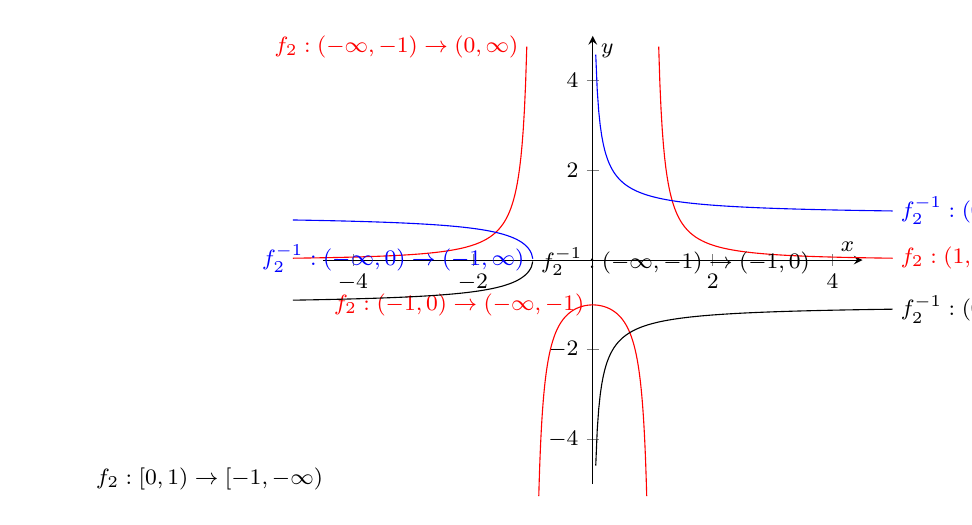
\begin{tikzpicture}
    \begin{axis}[
     axis lines=middle,clip=false,
            xmin=-4.5,xmax=4.5, ymin=-5,ymax=5,
            xticklabel style={black},
            xlabel=$x$,
            ylabel=$y$]
    \addplot[domain=-5:-1.1,samples=200,red]{1/(x^2-1)}
    node[left,pos=1.,font=\footnotesize]{$f_2:(-\infty, -1) \to (0,\infty)$};
    \addplot[domain=-0.9:0,samples=200,red]{1/(x^2-1)}
    node[left,pos=1.,font=\footnotesize]{$f_2:(-1,0) \to (-\infty, -1)$};
    \addplot[domain=0:0.9,samples=200,red]{1/(x^2-1)};
    node[left,pos=1.,font=\footnotesize]{$f_2:[0,1) \to [-1,-\infty)$};
    \addplot[domain=1.1:5,samples=200,red]{1/(x^2-1)}
    node[right,pos=1.,font=\footnotesize]{$f_2:(1,\infty) \to (0,\infty)$};
    \addplot[domain=-5:-1.001,samples=200,blue]{sqrt((1+x)/x)}
    node[left,pos=1.,font=\footnotesize]{$f_2^{-1}:(-\infty,0) \to (-1,\infty)$};
    \addplot[domain=0.05:5,samples=200,blue]{sqrt((1+x)/x)}
    node[right,pos=1.,font=\footnotesize]{$f_2^{-1}:(0,\infty) \to (1,\infty)$};
    \addplot[domain=-5:-1.001,samples=200,black]{-sqrt((1+x)/x)}
    node[right,pos=1.,font=\footnotesize]{$f_2^{-1}:(-\infty,-1) \to (-1,0)$};
    \addplot[domain=0.05:5,samples=200,black]{-sqrt((1+x)/x)}
    node[right,pos=1.,font=\footnotesize]{$f_2^{-1}: (0,\infty) \to (-\infty,-1)$};
    \end{axis}
\end{tikzpicture}
\newpage

\item
Die Funktion $\arcsin(x)$ ist die Umkehrfunktion von $\sin(x)$, wenn nur der Hauptwert betrachtet wird.
Nach Definition, schr\"anken wir den Definitionsbereich von $\sin(x)$ ein auf $-\frac{\pi}{2} \leq x \leq \frac{\pi}{2}$, 
w\"ahrend der Wertebereich $[-1,1]$ ist.
Die erste Ableitung von $\sin(x)$ ist $\cos(x) \geq 0$ f\"ur alle $x \in [-\frac{\pi}{2},\frac{\pi}{2}]$,
daher ist die Funktion monoton steigend und folglich injektiv.
Als Abbildung $f_3 : [-\frac{\pi}{2},\frac{\pi}{2}] \to [-1,1]$ ist die Funktion bijektiv.
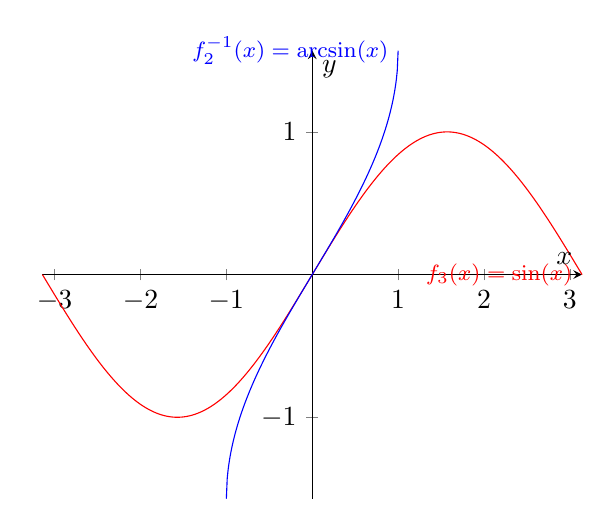
\begin{tikzpicture}
    \begin{axis}[
     axis lines=middle,clip=false,
            xmin=-pi,xmax=pi, ymin=-pi/2,ymax=pi/2,
            xticklabel style={black},
            xlabel=$x$,
            ylabel=$y$]
    \addplot[domain=-pi:pi,samples=200,red]{sin(deg(x))}
    node[left,pos=1.,font=\footnotesize]{$f_3(x)=\sin(x)$};
    \addplot[domain=-1:1,samples=200,blue]{asin(x)/180*pi}
    node[left,pos=1.,font=\footnotesize]{$f_2^{-1}(x)=\arcsin(x)$};
    \end{axis}
\end{tikzpicture}
\newpage
\item
Die Funktion $\arctan(x)$ ist die Umkehrfunktion von $\tan(x)$, wenn nur der Hauptwert betrachtet wird. 
Nach Definition beschr\"anken wir den Definitionsbereich von $\tan(x)$ auf $-\frac{\pi}{2}< x <\frac{\pi}{2}$, 
w\"ahrend der Wertebereich $(-\infty,\infty)$ ist.
Die erste Ableitung von $\tan(x)$ ist $\frac{1}{\cos^2(x)} > 0$ f\"ur alle $x \in (-\frac{\pi}{2},\frac{\pi}{2})$, daher ist die Funktion 
monoton steigend und folglich injektiv. 
Als Abbildung $f_3 : (-\frac{\pi}{2},\frac{\pi}{2}) \to (-\infty,\infty)$ ist sie bijektiv
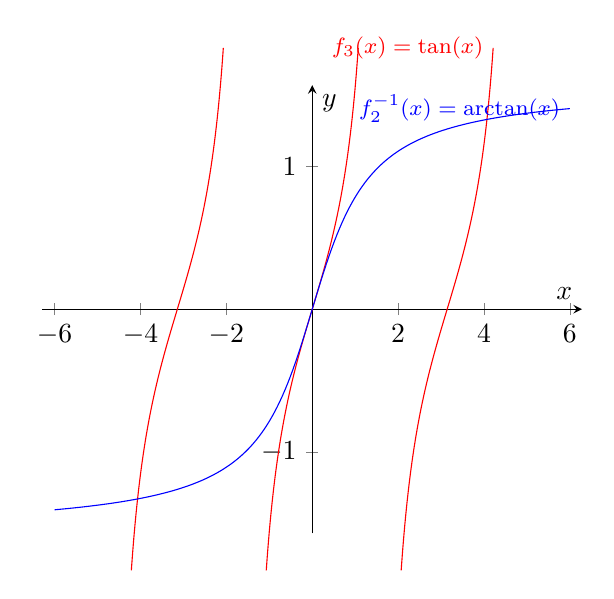
\begin{tikzpicture}
    \begin{axis}[
     axis lines=middle,clip=false,
            xmin=-2*pi,xmax=2*pi, ymin=-pi/2,ymax=pi/2,
            xticklabel style={black},
            xlabel=$x$,
            ylabel=$y$]
    \addplot[domain=-pi/2+0.5:pi/2-0.5,samples=200,red]{tan(deg(x))};
    \addplot[domain=-3*pi/2+0.5:-pi/2-0.5,samples=200,red]{tan(deg(x))};
    \addplot[domain=pi/2+0.5:3*pi/2-0.5,samples=200,red]{tan(deg(x))}
    node[left,pos=1.,font=\footnotesize]{$f_3(x)=\tan(x)$};
    \addplot[domain=-6:6,samples=200,blue]{atan(x)/180*pi}
    node[left,pos=1.,font=\footnotesize]{$f_2^{-1}(x)=\arctan(x)$};
    \end{axis}
\end{tikzpicture}
%clear all
%close all
%
%f=@(x) exp(1./x)
%
%% plot function and inverse branches
%
%% pt. I
%a=-3; b=-.01;
%
%x=linspace(a,b,100)';
%y=f(x);
%
%figure, plot(x,y,'LineWidth',2), hold on, grid, plot(y,x,'LineWidth',2), axis equal
%
%% pt. II
%a=.8; b=3.5;
%
%x=linspace(a,b,100)';
%y=f(x);
%
%figure, plot(x,y,'LineWidth',2), hold on, grid, plot(y,x,'LineWidth',2), axis equal

%clear all
%close all
%
%f=@(x) 1./(x.*x-1)
%
%% plot function and inverse branches
%
%% pt. I
%a=-10; b=-1.1;
%
%x=linspace(a,b,100)';
%y=f(x);
%
%figure, plot(x,y,'LineWidth',2), hold on, grid, plot(y,x,'LineWidth',2), axis equal
%
%% pt. II
%a=-.9; b=-.01;
%
%x=linspace(a,b,100)';
%y=f(x);
%
%figure, plot(x,y,'LineWidth',2), hold on, grid, plot(y,x,'LineWidth',2), axis equal
%
%% pt. III
%a=0; b=.9;
%
%x=linspace(a,b,100)';
%y=f(x);
%
%figure, plot(x,y,'LineWidth',2), hold on, grid, plot(y,x,'LineWidth',2), axis equal
%
%% pt. IV
%a=1.1; b=10;
%
%x=linspace(a,b,100)';
%y=f(x);
%
%figure, plot(x,y,'LineWidth',2), hold on, grid, plot(y,x,'LineWidth',2), axis equal

\end{iii}
}



\ifthenelse{\boolean{mitLoes}}{\ruleBig \cleardoublepage}
\Aufgabe[e]{Umkehrfunktion}{
Gegeben seien die folgenden Funktionen. Geben Sie den Definitionsbereich an (betrachten Sie dabei den Hauptwert der Funktion) 
und überprüfen Sie, ob die Funktionen invertierbar sind. Bestimmen Sie jeweils die inverse Funktion.
\begin{iii}
\item  
$f(x)=2x -1 $.
\item 
$f(x) = x^\frac{1}{3} $.
\item 
$f(x) = (x-1)^\frac{1}{3}$.
\item 
$f(x) = \dfrac{x}{x+1}$.
\item 
$f(x) = \log_2(x+3)$.
\item 
$f(x) = 2+\operatorname{e}^{x-1}$.
\item 
$f(x) = \arccos(x^{-2})$.
\end{iii}
}
\Loesung{
\begin{iii}
\item Die Funktion $f:\mathbb R \to \mathbb R$, 
$f(x)=2x -1$ ist bijektiv und daher invertierbar. Um die Umkehrfunktion zu bestimmen, l\"ost man die Gleichung
$y=\dfrac{x+1}{2}$ f\"ur die Variable $x$. Es gilt
\begin{align*}
2x-1 &= y,\\
2x &= y+1,\\
x&= \frac{y+1}{2}.
\end{align*}
Das Ergebnis erhalten wir durch Vertauschen der Variablennamen. Beide Funktionen sind auf dem Definitionsbereich $\mathbb R$
definiert.
\item Die Funktion
$x^\frac{1}{3}$ ist definiert f\"ur $x\in \mathbb R$. F\"ur die erste Ableitung gilt $\frac{1}{3}x^{-2/3}\ge 0$ f\"ur $x\in \mathbb R$, 
daher ist die Funktion streng monoton steigend und folglich injektiv. Au\ss erdem ist die Funktion surjektiv auf $\mathbb R$, weil sie nicht beschr\"ankt ist.
Daher ist die Funktion bijektiv und damit invertierbar. Die Umkehrfunktion $x^3$ hat den gleichen Definitionsbereich $\mathbb R$.
\item Die Funktion $(x-1)^{1/3}$ ist ebenso wie die vorherige Funktion bijektiv. Die Umkehrfunktion kann berechnet werden durch
\begin{align*}
(x-1)^\frac{1}{3} &= y,\\
x-1 & = y^3,\\
x = y^3+1
\end{align*}
mit dem Definitionsbereich $\mathbb R$.
\item Die Funktion $\displaystyle \frac{x}{x+1}$ ist definiert f\"ur $\mathbb R \setminus \{-1\}$. Die Funktion hat die Grenzwerte
$$\lim_{x\to\pm\infty} f(x)=1.$$
Daher ist sie surjektiv auf dem Wertebereich $(-\infty,1) \cup (1, +\infty)$. Die Funktion $f$ ist eine bijektive Abbildung
$f: (-\infty,-1) \cup (-1, +\infty)\to(-\infty,1) \cup (1, +\infty)$. Da die Ableitung $$f'(x)=\frac{1}{(x+1)^2} > 0, \quad \mathbb R \setminus \{-1\}$$
stets positiv ist, ist die Funktion streng monoton steigend auf dem Definitionsbereich.
Die Umkehrfunktion wird berechnet durch
\begin{align*}
\frac{x}{x+1} &= y\\
x & = (x+1)y\\
x(1-y) & = y\\
x &= \frac{y}{1-y},
\end{align*}
Die Funktion ist definiert f\"ur $x \in \mathbb R \setminus \{+1\}$.
\item Die Funktion $\log_2(x+3)$ ist definiert f\"ur $x+3 > 0 \Rightarrow x > -3$. Sie ist streng monoton steigend. Die Abbildung $f: (-3, +\infty) \to \mathbb R$ 
ist bijektiv.
Die Umkehrfunktion kann berechnet werden als
\begin{align*}
\log_2(x+3) &= y,\\
2^{\log_2(x+3)} & = 2^y,\\
x+3 = 2^y,\\
x = 2^y-3,
\end{align*}
Die Funktion ist definiert auf $\mathbb R$ und der Wertebereich ist $(-3, +\infty)$.
\item Die Funktion $2+\operatorname{e}^{x-1}$ ist definiert auf $x\in \mathbb R$. Die Abbildung $f: \mathbb R \to (2, +\infty)$ ist bijektiv,
weil die Ableitung stets positiv ist $f'(x) = \operatorname{e}^{x-1} > 0$.
%
Die Umkehrfunktion ist
\begin{align*}
2+\operatorname{e}^{x-1} &= y\\
\operatorname{e}^{x-1} & = y-2\\
\ln{\operatorname{e}^{x-1}}& = \ln{(y-2)}\\
x & = \ln{(y-2)}+1,
\end{align*}
welche definiert ist auf $x\in (2, +\infty)$ und der Wertebereich ist $\mathbb R$.
\item Die Funktion $\arccos(x)$ ist die Umkehrfunktion von $\cos(x)$, wenn man nur den Hauptwert der Funktion betrachtet. Nach Definition beschr\"anken wir den 
Definitionsbereich von $\cos(x)$ auf $0 \leq x \leq \pi$, dann ist der Wertebereich $[-1,1]$. Damit ist der Definitionsbereich von $\arccos(x)$ gegeben 
durch $[-1,1]$ und der Wertebereich ist $[0,\pi]$. F\"ur die Funktion $\arccos(x^{-2})$ ist der Definitionsbereich der Definitionsbereich der 
zusammengesetzten Funktion. Der Definitionsbereich der inneren Funktion $x^{-2}$ ist $\mathbb R \setminus \{0\}$. Der Definitionsbereich der 
\"au\ss eren Funktion $\arccos(w)$ wie oben bemerkt, ist $w\in[-1,1]$, daher muss $w:=x^{-2}\geq-1$ gelten, was immer wahr ist. Es gilt
$x^{-2} \leq 1 \Rightarrow x^2 \ge 1 \Rightarrow x \ge 1 \land x \leq -1$. Der Wertebereich der zusammengesetzten Funktion $\arccos(x^{-2})$ ist $[0,\pi]$, weil das 
der Wertebereich der \"au\ss eren Funktion ist.\\
Zu untersuchen bleibt die Monotonie der zusammengesetzten Funktion. Da die Funktion $x^{-2}$ nicht-monoton ist, k\"onnen wir daraus keine Aussage \"uber 
die Monotonie der zusammengesetzten Funktion treffen. Die Ableitung von $\arccos$ ist
$$(\arccos(w))' = -\frac{1}{\sqrt{1-w^2}}.$$
F\"ur die Ableitung der zusammengesetzten Funktion benutzen wir die Kettenregel. Damit erhalten wir die Ableitung
\begin{align*}
\left(\arccos(x^{-2})\right)^\prime & = -\frac{1}{\sqrt{1-(x^{-2})^2}}\, (-2 x^{-3}),\\
& = \frac{2}{\sqrt{1-(x^{-4})}}\, x^{-3},
\end{align*}
welche ungerade ist. Daher ist die zusammengesetzte Funktion $\arccos(x^{-2})$ nicht-monoton. Um die Umkehrfunktion zu bestimmen m\"ussen wir den Definitionsbereich
in zwei Teile teilen, in denen die Funktion jeweils monoton ist. Damit definieren wir zwei Zweige der Funktion. Die Funktion ist monoton, wenn wir sie auf den Definitionsbereich 
f\"ur den $x$-positiven Zweig auf $[1, \infty)$ einschr\"anken und f\"ur den $x$-negativen Zweig auf $(-\infty, -1]$ einschr\"anken. 
Die Umkehrfunktion wird berechnet durch
\begin{align*}
\arccos(x^{-2}) &= y,\\
\cos(\arccos{x^{-2}}) & = \cos(y),\\
x^{-2} & = \cos(y),\\
x & = \pm \frac{1}{\sqrt{\cos(y)}}.
\end{align*}
Durch Vertauschen der Variablennamen erhalten wir die Umkehrfunktion
$$
y = \pm \frac{1}{\sqrt{\cos(x)}}.
$$
Diese Funktion ist die zusammengesetzte Funktion mit dem Definitionsbereich, der die Bedingungen $$\cos(x)>0$$ und $x\in [0, \pi]$ erf\"ullt. 
Dies ist der Definitionsbereich f\"ur den Hauptwert von $\cos(x)$. Daraus ergibt sich die Bedingung $x\in [0,\frac{\pi}{2})$.  Der Wertebereich ist der Wertebereich der \"au\ss eren Funktion.
Also $[1, +\infty]$ f\"ur den positiven Zweig und  $(-\infty, -1]$ f\"ur den negativen Zweig.
\end{iii}
}

\ErgebnisC{InverseFunktion}{
\textbf{i}) $f^{-1}(x)=\dfrac{x+1}{2}.$
\textbf{ii}) $f^{-1}(x) = x^3.$
\textbf{iii}) $f^{-1}(x) = x^3+1.$
\textbf{iv}) $f^{-1}(x) = \dfrac{x}{1-x}.$
\textbf{v}) $f^{-1}(x) = 2^x-3.$
\textbf{vi}) $f^{-1}(x) = \ln(x-2) + 1.$
\textbf{vii}) $f^{-1}(x) = \pm\dfrac{1}{\sqrt{\cos{x}}}.$
}

\ifthenelse{\boolean{mitLoes}}{\ruleBig \cleardoublepage}
\Aufgabe[e]{Inverse Funktion}{
%Verify that the given pairs of functions are inverse pairs. Specify their domain (consider the principal value if needed) and check if they are invertible.
Gegeben seien die folgenden Funktionen
\begin{multicols}{2}
\begin{iii}
\item  
$f_1(x)=\operatorname{e}^{\frac{1}{x}}$,
\item 
$f_2(x)=\frac{1}{x^2-1}$,
\item 
$f_3(x)=\sin(x)$,
\item 
$f_4(x)=\tan(x)$.
\end{iii}
\end{multicols}
\begin{abc}
\item Bestimmen Sie den maximalen Definitionsbereich und den Wertebereich.
\item Betimmen Sie die Einschr\"ankung des Definitionsbereichs und Wertebereichs, so dass die Funktionen bijektiv sind. 
(Betrachten Sie, falls n\"otig, den Hauptzweig.)
\item Bestimmen Sie die inverse Funktion.
\item Skizzieren Sie die Funktion sowie deren inverse Funktion.
\end{abc}
}
\Loesung{
\begin{iii}
\item
The function $f_1(x)=\operatorname{e}^{\frac{1}{x}}$ is defined for $x\in \mathbb{R}\setminus\{0\}$. 
The first derivative is $-\frac{1}{x^2}\operatorname{e}^{\frac{1}{x}}<0$ for all $x\in \mathbb{R}\setminus\{0\}$ therefore $f_1$ is strictly monotonically decreasing on each branch, thus injective.
The function has the limit
$$
\lim_{x\to \pm \infty} f_1(x) = 1.
$$
therefore it is surjective on the codomain $ (0,1)\cup (1,\infty)$.
The function $f_1$ is bijective as a map $f_1:\mathbb{R}\setminus\{0\} \to (0,1) \cup (1,\infty)$.
The inverse function can be computed as
\begin{align*}
\operatorname{e}^{\frac{1}{x}}=y, 
\quad y = \begin{cases}(0, 1) & \text{for} x <0,
                       (1, \infty) \text {for} x>0,\end{cases}\\
\frac{1}{x} =\ln(y),\\
x=\frac{1}{\ln(y)}, \quad (\ln(y) \neq 0).
\end{align*}
A change of the variable names gives the inverse function 
$$f_1^{-1}(x)=\frac{1}{\ln(x)}.$$

\begin{tikzpicture}
    \begin{axis}[
     axis lines=middle,clip=false,
            xmin=-4.5,xmax=4.5, ymin=-5,ymax=5,
            xticklabel style={black},
            xlabel=$x$,
            ylabel=$y$]
    \addplot[domain=-5:-0.0001,samples=200,red]{exp(1/x)}
    node[left,pos=1.,font=\footnotesize]{$f_1: (-\infty,0) \to (0,1)$};
    \addplot[domain=0.5:5,samples=200,red]{exp(1/x)}
    node[right,pos=1.,font=\footnotesize]{$f_1: (0,\infty) \to (1,\infty)$};
    \addplot[domain=0.0001:0.8,samples=200,blue]{1/(ln(x))}
    node[right,pos=1.,font=\footnotesize]{$f_1^{-1}: (0,1) \to (\infty,0)$};
    \addplot[domain=1.2:5,samples=200,blue]{1/(ln(x))}
    node[right,pos=1.,font=\footnotesize]{$f_1^{-1}: (1,\infty) \to (0,\infty)$};
\end{axis}
\end{tikzpicture}
\newpage
\item
The function $f_2(x) = \frac{1}{x^2-1}$ is not defined for $x = \pm 1$.
The domain of definition is $(-\infty,-1) \cup (-1,1) \cup (1,\infty)$.
The codamain is $(-\infty,1] \cup (0,\infty)$. 
The first derivative 
$$
f_2'(x) = -\frac{2x}{(x^2 - 1)^2}
$$
is positive for $x \in (-\infty, -1)$ and $x \in (-1,0)$ therefore monotonically increasing and 
it is negative for $x \in (0,1)$ and $x \in (1,\infty)$ therefore monotonically decreasing. 
The maps $f_2 : (0,1) \to (-\infty,1] \cup (1,\infty) \to \cup (0,\infty)$ is bijective and the inverse function
can be computed as
\begin{align*}
\frac{1}{x^2-1}=y,\\
x^2-1 = \frac{1}{y},\\
x^2 = \frac{1}{y} + 1,\\
x = \sqrt{\frac{1}{y} + 1}.
\end{align*}
A change of the variable names gives the inverse function 
$$f_2^{-1}(x)=\sqrt{\frac{1+x}{x}}.$$
Analogous we can invert the negative branch. We restrict the domain of definition to $(-\infty,-1)\cup(-1,0)$.
The map $f_2: (-\infty,-1)\cup(-1,0) \to (-\infty,-1]\cup (0,\infty)$ is bijective and the inverse function
can be computed as above, but we take the negative square root. The inverse function of negative branch is:
$$f_2^{-1}(x)=\sqrt{\frac{1}{x}+1}.$$
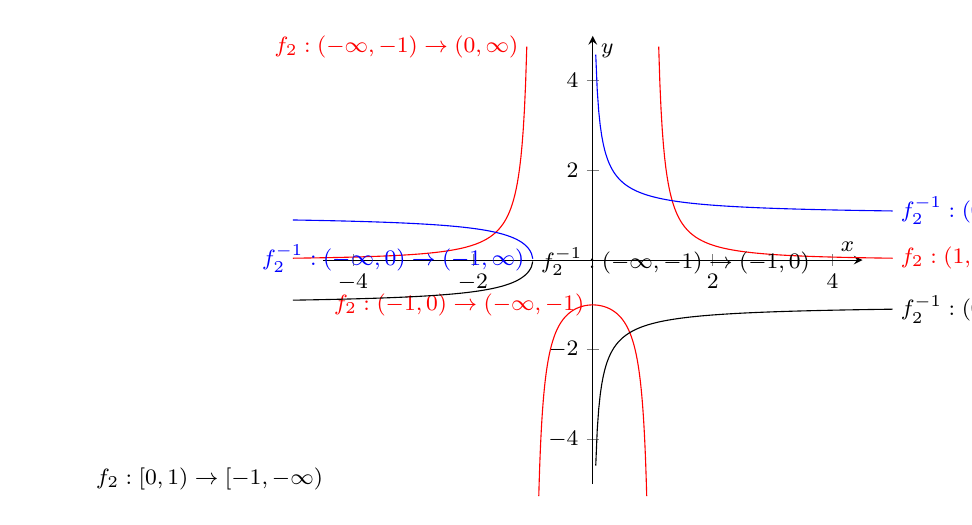
\begin{tikzpicture}
    \begin{axis}[
     axis lines=middle,clip=false,
            xmin=-4.5,xmax=4.5, ymin=-5,ymax=5,
            xticklabel style={black},
            xlabel=$x$,
            ylabel=$y$]
    \addplot[domain=-5:-1.1,samples=200,red]{1/(x^2-1)}
    node[left,pos=1.,font=\footnotesize]{$f_2:(-\infty, -1) \to (0,\infty)$};
    \addplot[domain=-0.9:0,samples=200,red]{1/(x^2-1)}
    node[left,pos=1.,font=\footnotesize]{$f_2:(-1,0) \to (-\infty, -1)$};
    \addplot[domain=0:0.9,samples=200,red]{1/(x^2-1)};
    node[left,pos=1.,font=\footnotesize]{$f_2:[0,1) \to [-1,-\infty)$};
    \addplot[domain=1.1:5,samples=200,red]{1/(x^2-1)}
    node[right,pos=1.,font=\footnotesize]{$f_2:(1,\infty) \to (0,\infty)$};
    \addplot[domain=-5:-1.001,samples=200,blue]{sqrt((1+x)/x)}
    node[left,pos=1.,font=\footnotesize]{$f_2^{-1}:(-\infty,0) \to (-1,\infty)$};
    \addplot[domain=0.05:5,samples=200,blue]{sqrt((1+x)/x)}
    node[right,pos=1.,font=\footnotesize]{$f_2^{-1}:(0,\infty) \to (1,\infty)$};
    \addplot[domain=-5:-1.001,samples=200,black]{-sqrt((1+x)/x)}
    node[right,pos=1.,font=\footnotesize]{$f_2^{-1}:(-\infty,-1) \to (-1,0)$};
    \addplot[domain=0.05:5,samples=200,black]{-sqrt((1+x)/x)}
    node[right,pos=1.,font=\footnotesize]{$f_2^{-1}: (0,\infty) \to (-\infty,-1)$};
    \end{axis}
\end{tikzpicture}
\newpage

\item
The function $\arcsin(x)$ is the inverse function of $\sin(x)$ considering only the principal branch.
By definition, we restrict the domain of definition of $\sin(x)$ in $-\frac{\pi}{2} \leq x \leq \frac{\pi}{2}$, 
while the codomain is $[-1,1]$.
The first derivative of $\sin(x)$ is $\cos(x) \geq 0$ for all $x \in [-\frac{\pi}{2},\frac{\pi}{2}]$,
therefore it is monotonicallyincreasing, thus injective.
As map $f_3 : [-\frac{\pi}{2},\frac{\pi}{2}] \to [-1,1]$ it is bijective.
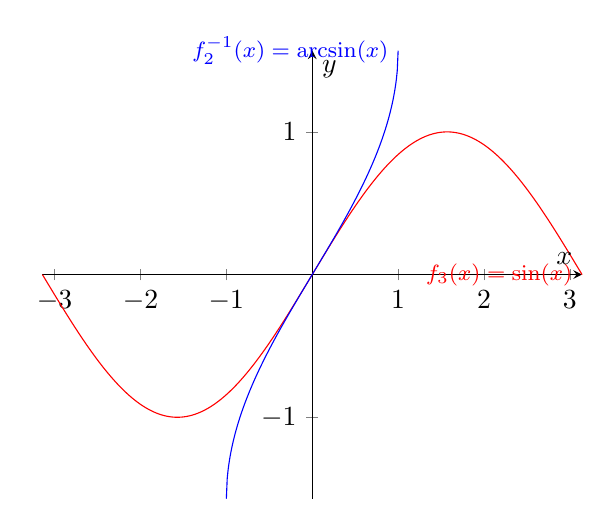
\begin{tikzpicture}
    \begin{axis}[
     axis lines=middle,clip=false,
            xmin=-pi,xmax=pi, ymin=-pi/2,ymax=pi/2,
            xticklabel style={black},
            xlabel=$x$,
            ylabel=$y$]
    \addplot[domain=-pi:pi,samples=200,red]{sin(deg(x))}
    node[left,pos=1.,font=\footnotesize]{$f_3(x)=\sin(x)$};
    \addplot[domain=-1:1,samples=200,blue]{asin(x)/180*pi}
    node[left,pos=1.,font=\footnotesize]{$f_2^{-1}(x)=\arcsin(x)$};
    \end{axis}
\end{tikzpicture}
\newpage
\item
The function $\arctan(x)$ is the inverse function of $\tan(x)$ considering only the principal branch. 
By definition, we restrict the domain of $\tan(x)$ in $-\frac{\pi}{2}< x <\frac{\pi}{2}$, 
while the codomain is $(-\infty,\infty)$.
The first derivative of $\tan(x)$ is $\frac{1}{\cos^2(x)} > 0$ for all $x \in (-\frac{\pi}{2},\frac{\pi}{2})$, therefore it is monotonically
increasing, thus injective. As map $f_3 : (-\frac{\pi}{2},\frac{\pi}{2}) \to (-\infty,\infty)$ it is bijective.
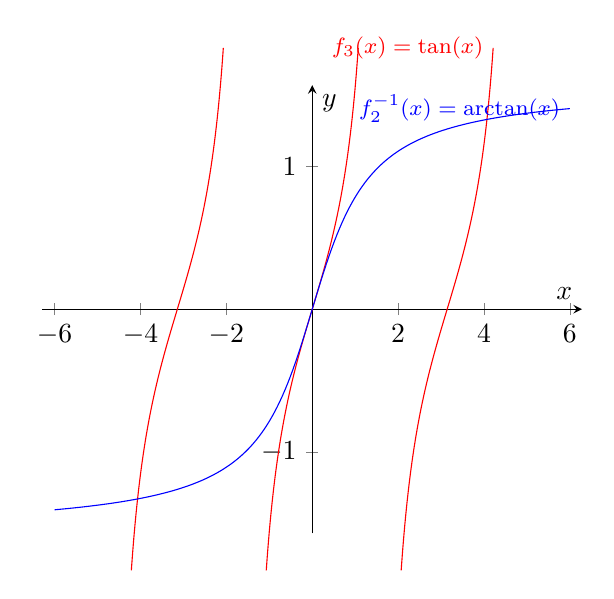
\begin{tikzpicture}
    \begin{axis}[
     axis lines=middle,clip=false,
            xmin=-2*pi,xmax=2*pi, ymin=-pi/2,ymax=pi/2,
            xticklabel style={black},
            xlabel=$x$,
            ylabel=$y$]
    \addplot[domain=-pi/2+0.5:pi/2-0.5,samples=200,red]{tan(deg(x))};
    \addplot[domain=-3*pi/2+0.5:-pi/2-0.5,samples=200,red]{tan(deg(x))};
    \addplot[domain=pi/2+0.5:3*pi/2-0.5,samples=200,red]{tan(deg(x))}
    node[left,pos=1.,font=\footnotesize]{$f_3(x)=\tan(x)$};
    \addplot[domain=-6:6,samples=200,blue]{atan(x)/180*pi}
    node[left,pos=1.,font=\footnotesize]{$f_2^{-1}(x)=\arctan(x)$};
    \end{axis}
\end{tikzpicture}
\textbf{d)} 
The MATLAB code for the plots of the functions and their inverse functions can be found in the ILIAS.

%clear all
%close all
%
%f=@(x) exp(1./x)
%
%% plot function and inverse branches
%
%% pt. I
%a=-3; b=-.01;
%
%x=linspace(a,b,100)';
%y=f(x);
%
%figure, plot(x,y,'LineWidth',2), hold on, grid, plot(y,x,'LineWidth',2), axis equal
%
%% pt. II
%a=.8; b=3.5;
%
%x=linspace(a,b,100)';
%y=f(x);
%
%figure, plot(x,y,'LineWidth',2), hold on, grid, plot(y,x,'LineWidth',2), axis equal

%clear all
%close all
%
%f=@(x) 1./(x.*x-1)
%
%% plot function and inverse branches
%
%% pt. I
%a=-10; b=-1.1;
%
%x=linspace(a,b,100)';
%y=f(x);
%
%figure, plot(x,y,'LineWidth',2), hold on, grid, plot(y,x,'LineWidth',2), axis equal
%
%% pt. II
%a=-.9; b=-.01;
%
%x=linspace(a,b,100)';
%y=f(x);
%
%figure, plot(x,y,'LineWidth',2), hold on, grid, plot(y,x,'LineWidth',2), axis equal
%
%% pt. III
%a=0; b=.9;
%
%x=linspace(a,b,100)';
%y=f(x);
%
%figure, plot(x,y,'LineWidth',2), hold on, grid, plot(y,x,'LineWidth',2), axis equal
%
%% pt. IV
%a=1.1; b=10;
%
%x=linspace(a,b,100)';
%y=f(x);
%
%figure, plot(x,y,'LineWidth',2), hold on, grid, plot(y,x,'LineWidth',2), axis equal

\end{iii}
}



\ifthenelse{\boolean{mitLoes}}{\ruleBig \cleardoublepage}
\Aufgabe[e]{Umkehrfunktion}{
\begin{abc}
\item[e] Geben Sie zu den folgenden Funktionen an, in welchem Bereich sie umkehrbar sind, geben Sie im Punkt
$(0,f_j(0))$ den Wert der Ableitung von $f_j^{-1}(x)$ an. 
\begin{align*}
f_1(y)=& y^3-3y\\
f_2(y)=& \frac{y^2+3y}{1-y}
\end{align*}
\item Gegeben seien die Funktionen 
$$g_3(x)=\tan(x),\qquad g_4(x)=\EH{x^2+2x-8},\qquad g_5(x)=\cosh(x),\qquad g_6(x)=\frac 1{x^2+2}.$$
Bestimmen Sie zun\"achst die Ableitungen $g_j'(x)\, (j=3,4,5,6)$ dieser Funktionen. \\
Ermitteln Sie daraus mit Hilfe von Satz 3.38 (Ableitung der Umkehrfunktion) die Ableitung der
Umkehrfunktionen $f_j(y)=g_j^{-1}(x)\,(j=3,4,5,6)$. (Es gilt $f_j(g_j(x))=x$.)\\
%\begin{align*}
%f_3(y)=\arctan(y),&\quad&f_4^{-1}(x)=\EH{x^2+2x-8},& \quad & f_5(y)=\mathrm{Ar\, cosh} y ,&\quad& f_6(y)=\sqrt{\frac 1 y -2}
%\end{align*}
Geben Sie auch f\"ur jede Funktion an, in welchem Bereich die Umkehrfunktion erkl\"art ist. 
\end{abc}


}


\Loesung{
\begin{abc}
\item \begin{iii}
\item Die Ableitung der ersten Funktion ist $f_1'(y)=3y^2-3$, diese wird Null bei $y=\pm 1$. Im
Intervall $[-1,1]$ ist $f_1$ also streng monoton und damit umkehrbar.\\
Die Ableitung der Umkehrfunktion bei $(0,f_1(0))=(0,0)$ ist 
$$(f_1^{-1})'(0)=\frac 1{f_1'(0)}=\frac 1{-3}=-\frac 13.$$
\item Wie schon in Aufgabe 1 festgestellt, ist die Funktion $f_2$ im Invervall $[-1,1[$ streng monoton
steigend und damit umkehrbar. Die Ableitung wurde dort ebenfalls berechnet und es ist
$$f_2'(0)=3 \text{ und }f_2(0)=0.$$
Also ist die Ableitung der Umkehrfunktion im Ursprung 
$$(f_2^{-1})'(0)=\frac 1{f_2'(0)}=\frac 13.$$
\end{iii}
\item \begin{iii}\setcounter{enumii}{2}
\item Die Funktion $g_3(x)=\tan(x)$ ist auf dem Intervall $]-\pi/2,\pi/2[$ umkehrbar. Ihre Umkehrfunktion ist 
$$f_4=\arctan:\, \R\rightarrow ]-\pi/2,\pi/2[.$$
Zun\"achst folgt mit der Quotientenregel 
$$g_3'(x)=\left(\frac{\sin(x)}{\cos(x)}\right)'=\frac{\cos^2(x)+\sin^2(x)}{\cos^2(x)}=\frac
1{\cos^2(x)}.$$
Die Ableitung von $f_4(y)=\arctan(y)$ ergibt sich daraus mit Hilfe des angegebenen Satzes: 
\begin{align*}
\arctan'(y)=&\left.\frac 1{\tan'(x)}\right|_{x=\arctan(y)}\\
=&\left.\frac 1{\frac 1{\cos^2(x)}}\right|_{x=\arctan(y)}
= \left.\frac 1{\frac{\sin^2(x)}{\cos^2(x)}+\frac{\cos^2(x)}{\cos^2(x)}}\right|_{x=\arctan(y)}\\
=& \left.\frac 1{\tan^2(x) + 1}\right|_{x=\arctan(y)}
=\frac 1 {\tan^2(\arctan(y))+1}\\
=&  \frac 1{1+y^2}.
\end{align*}
\item Die Ableitung der Funktion $g_4(x)$ ist 
$$g_4'(x)=(2x+2)\EH{x^2+2x-8}.$$
Sie ist gr\"oßer Null f\"ur $x>-1$, also ist die Funktion 
$$g_4: [-1,\infty[\rightarrow [\EH{-9},\infty[$$
invertierbar. \\
Dort ist mit Satz 3.38
$$f_4'(y)=\frac{1}{g_4'(f_4(y))}=\left.\frac{\EH{8-x^2-2x}}{2x+2}\right|_{x=f_4(y)} =\left.\frac{1}{g_4(x)(2x+2)}\right|_{x=f_4(y)}$$
und außerdem ist $f_4(y)=\sqrt{\ln y +9}-1$ f\"ur $y\geq\EH {-9}$.
Insgesamt hat man damit
$$f_4'(y)=\frac{1}{2y\sqrt{\ln y + 9}}.$$
\item Der $\cosh$ ist auf der rechten reellen Halbgraden $[0,\infty[$ umkehrbar und hat die
Ableitung
$$g_5'(x)=\sinh(x).$$
Damit hat man f\"ur 
$$f_5=\text{Ar cosh}:[1,\infty[\rightarrow [0,\infty[$$ 
die Ableitung
\begin{align*}
\text{Ar cosh}'(y)=&\frac 1{\cosh'(\text{Ar cosh}y)}=\frac{1}{\sinh(\text{Ar cosh}y)}\\
=& \frac 1{\sqrt{\cosh^2(\text{Ar cosh}y)-1}}=\frac 1{\sqrt{y^2-1}}.
\end{align*}
Man beachte, dass wegen $x=\text{Ar cosh} y>0$ gilt: $\sinh x = +\sqrt{\cosh^2x-1}$. 
\item Die Funktion $g_6(x)=\frac 1{2+x^2}$ hat die Ableitung
$$g_6'(x)=\frac{-2x}{(2+x^2)^2}.$$
F\"ur $x>0$ ist $g_6'(x)<0$. Also ist $g_6$ dort monoton fallend und invertierbar mit 
$$g_6:[0,\infty[\rightarrow \left]0,\frac 12\right]$$
bzw. 
$$f_6:\left]0,\frac 12\right]\rightarrow[0,\infty[,\quad f_6(y)=\sqrt{\frac 1 y -2}.$$
Die Ableitung der Umkehrfunktion ergibt sich zu 
\begin{align*}
f_6'(y)=&\frac 1{g_6'(f_6(y))}=-\left.\frac{(2+x^2)^2}{2x}\right|_{x=f_6(y)}\\
=& -\frac{\left( 2 + 1/y-2\right)^2}{2\sqrt{1/y-2}}=-\frac{1}{2\sqrt{y^3-2y^4}}.
\end{align*}
\end{iii}
\end{abc}


}

\newcounter{AufganalysUmkeFunk001}
\setcounter{AufganalysUmkeFunk001}{\theAufg}
\Ergebnis{\subsubsection*{Ergebnisse zu Aufgabe \arabic{Blatt}.\arabic{AufganalysUmkeFunk001}:}
\textbf{ a)} $f_1^{-1}(0)=-1/3$, $f_2^{-1}(0)=1/3$
}

\ifthenelse{\boolean{mitLoes}}{\ruleBig \cleardoublepage}




\ifthenelse{\boolean{mitLoes}}{\cleardoublepage}{}
\ifthenelse{\boolean{mitErg}}{
\ruleBig
\Ergebnisse}{}


\end{twocolumn}
\end{document}
